\documentclass[11pt]{article}
\usepackage[margin=1in]{geometry}
\usepackage[T1]{fontenc}
\usepackage[utf8]{inputenc}
\usepackage{lmodern}
\usepackage{microtype}
\usepackage[dvipsnames]{xcolor}
\usepackage{amsmath,amssymb}
\usepackage{enumitem}
\usepackage{booktabs}
\usepackage{hyperref}
\usepackage{fancyhdr}
\usepackage{tikz}
\usepackage[most]{tcolorbox}
\usepackage{titlesec}
\usepackage{parskip}
\usepackage{array}
\usetikzlibrary{arrows.meta,positioning,calc,shapes.geometric}

\hypersetup{
  colorlinks=true,
  linkcolor=MidnightBlue,
  urlcolor=BrickRed,
  pdftitle={Machine Intelligence I --- Complete Lecture Notes},
  pdfauthor={Bodhi for Arjun Puri}
}

\definecolor{Ink}{HTML}{1F2430}
\definecolor{Muted}{HTML}{5E6879}
\definecolor{Accent}{HTML}{8B3D2E}
\definecolor{AccentBlue}{HTML}{0F5C73}
\definecolor{Paper}{HTML}{FAF7F2}
\definecolor{Soft}{HTML}{F2ECE2}
\definecolor{SoftBlue}{HTML}{EAF3F6}
\definecolor{SoftRose}{HTML}{F7EDEA}

\pagestyle{fancy}
\fancyhf{}
\fancyhead[L]{\textcolor{Muted}{Machine Intelligence I --- Lecture Notes}}
\fancyhead[R]{\textcolor{Muted}{Complete course}}
\fancyfoot[C]{\textcolor{Muted}{\thepage}}
\setlength{\headheight}{14pt}

\titleformat{\section}{\Large\bfseries\color{Ink}}{\thesection}{0.6em}{}
\titleformat{\subsection}{\large\bfseries\color{AccentBlue}}{}{0em}{}
\titleformat{\subsubsection}{\normalsize\bfseries\color{Accent}}{}{0em}{}

\newtcolorbox{summarybox}{
  colback=SoftBlue,
  colframe=AccentBlue!55,
  boxrule=0.6pt,
  arc=4mm,
  left=2mm,right=2mm,top=1.5mm,bottom=1.5mm
}

\newtcolorbox{conceptbox}[1]{
  colback=Soft,
  colframe=Accent!45,
  title=\textbf{#1},
  fonttitle=\color{Ink},
  boxrule=0.6pt,
  arc=4mm,
  left=2mm,right=2mm,top=1.5mm,bottom=1.5mm
}

\newcommand{\miheader}[1]{%
  {\Large\bfseries\color{Ink} #1}\par\vspace{0.35em}\color{Muted}\hrule height 0.6pt\color{black}\vspace{0.9em}
}

\begin{document}
\hypersetup{pageanchor=false}

\begin{titlepage}
  \pagecolor{Paper}
  \color{Ink}
  \centering
  \vspace*{1.3cm}

  {\small\textsc{Course lecture notes}}\par
  \vspace{0.55cm}
  {\Huge\bfseries Machine Intelligence I\\[0.25em] Lecture Notes}\par
  \vspace{0.35cm}
  {\Large Complete course synthesis with equations and intuition}\par
  \vspace{0.7cm}
  {\color{Muted}\rule{0.72\textwidth}{0.7pt}}\par
  \vspace{0.8cm}

  \begin{minipage}{0.82\textwidth}
  \centering
  {\large A LaTeX study guide synthesizing the full Machine Intelligence I lecture sequence from supervised learning foundations through Bayesian inference and reinforcement learning.}\par
  \vspace{0.9cm}
  \begin{summarybox}
    \textbf{Coverage}\par
    \vspace{0.15em}
    \begin{itemize}[leftmargin=1.4em,itemsep=0.24em]
      \item Learning paradigms, connectionist neurons, multilayer perceptrons, and optimization
      \item Deep learning, recurrent neural networks, and radial basis function networks
      \item Statistical learning theory and support vector machines
      \item Uncertainty, Bayesian networks, Bayesian model selection, and Bayesian prediction
      \item Reinforcement learning: value functions, Q-values, policy iteration, and exploration
    \end{itemize}
  \end{summarybox}
  \end{minipage}

  \vfill
  {\large Prepared for Arjun Puri}\par
  \vspace{0.18cm}
  {\normalsize\color{Muted} Generated in LaTeX with Bodhi \textbullet\ April 15, 2026}\par
\end{titlepage}
\hypersetup{pageanchor=true}

\pagenumbering{roman}
\tableofcontents
\clearpage
\pagenumbering{arabic}

\section*{Orientation}
\addcontentsline{toc}{section}{Orientation}
These notes now consolidate the full \emph{Machine Intelligence I} lecture arc into one narrative. The goal is not to reproduce every slide verbatim, but to extract the conceptual spine of the course: what kinds of learning problems exist, how neural and probabilistic models are built, how capacity and generalization are controlled, and how sequential decision-making is formalized.

\begin{summarybox}
\textbf{The big arc.} The course starts with supervised learning foundations and neural network building blocks, moves through optimization and deep architectures, then turns to capacity control and support vector machines, shifts into probabilistic reasoning and Bayesian inference, and concludes with reinforcement learning as sequential decision-making under uncertainty.
\end{summarybox}

\section{Introduction and learning paradigms}
\miheader{Why the course starts here}
Machine intelligence is framed as the study of \textbf{embedded agents}: systems that perceive the world, build internal representations, and choose actions. The opening contrast is intuitive and motivating:
\begin{itemize}[leftmargin=1.5em]
  \item \textbf{Brains} are strong at pattern recognition, language, inference, and adaptive control.
  \item \textbf{Machines} are strong at exact symbolic manipulation, arithmetic, and brute-force search.
\end{itemize}
The course goal is to design systems that \emph{learn} useful input--output relationships from data instead of being exhaustively hand-programmed.

\begin{center}
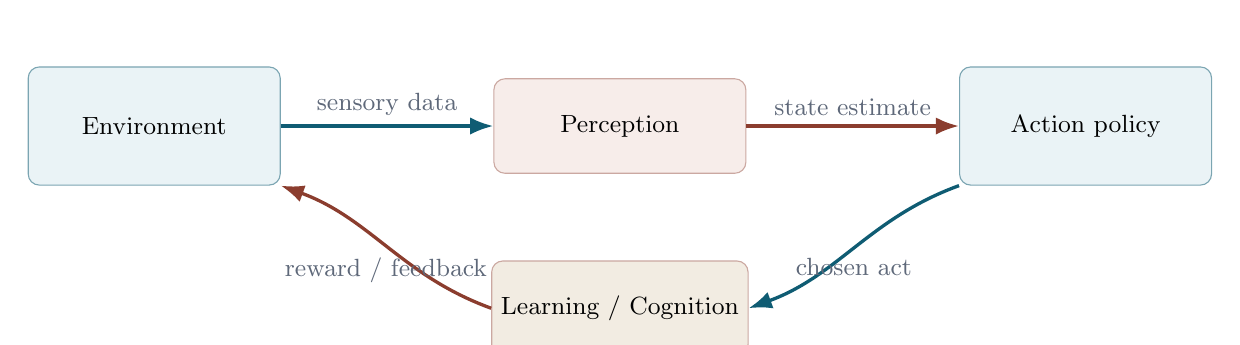
\begin{tikzpicture}[>=Latex, node distance=1.6cm, every node/.style={font=\small}]
  \node[draw=AccentBlue!55, fill=SoftBlue, rounded corners=4pt, minimum width=3.2cm, minimum height=1.5cm] (env) {Environment};
  \node[draw=Accent!45, fill=SoftRose, rounded corners=4pt, right=2.7cm of env, minimum width=3.2cm, minimum height=1.2cm] (per) {Perception};
  \node[draw=Accent!45, fill=Soft, rounded corners=4pt, below=1.1cm of per, minimum width=3.2cm, minimum height=1.2cm] (learn) {Learning / Cognition};
  \node[draw=AccentBlue!55, fill=SoftBlue, rounded corners=4pt, right=2.7cm of per, minimum width=3.2cm, minimum height=1.5cm] (act) {Action policy};
  \draw[->, very thick, AccentBlue] (env) -- node[above, text=Muted] {sensory data} (per);
  \draw[->, very thick, Accent] (per) -- node[above, text=Muted] {state estimate} (act);
  \draw[->, very thick, AccentBlue] (act.south west) to[out=-160,in=20] node[below, text=Muted] {chosen act} (learn.east);
  \draw[->, very thick, Accent] (learn.west) to[out=160,in=-20] node[below, text=Muted] {reward / feedback} (env.south east);
\end{tikzpicture}
\end{center}

\subsection{Learning as model selection}
A machine-learning pipeline can be understood as choosing three things:
\begin{enumerate}[leftmargin=1.6em]
  \item a \textbf{model class},
  \item a \textbf{performance measure}, and
  \item an \textbf{optimization procedure}.
\end{enumerate}
Learning is therefore not just ``fit a curve.'' It is: define a family of candidate hypotheses, define what counts as good performance, and search that family for a good solution.

\subsection{The three main paradigms}
\begin{conceptbox}{Supervised learning}
Learn a mapping from labeled examples $(x^{(\alpha)}, y^{(\alpha)})$. Typical tasks are classification and regression. The central question is: \emph{how should the model predict the target from the input?}
\end{conceptbox}

\begin{conceptbox}{Unsupervised learning}
Learn useful structure from inputs alone. Typical goals include clustering, density estimation, and dimensionality reduction. The central question is: \emph{what latent regularities are present in the data?}
\end{conceptbox}

\begin{conceptbox}{Reinforcement learning}
Learn behavior from interaction with an environment. Data arrive as trajectories over time rather than IID input--label pairs. The central question is: \emph{which action sequence maximizes expected future reward?}
\end{conceptbox}

\subsection{What matters conceptually}
\begin{itemize}[leftmargin=1.5em]
  \item Supervised learning is about \textbf{prediction from examples}.
  \item Unsupervised learning is about \textbf{structure without labels}.
  \item Reinforcement learning is about \textbf{sequential decision-making under delayed feedback}.
\end{itemize}

\section{Connectionist neurons}
\miheader{The basic computational unit}
A connectionist neuron is a mathematical abstraction of a biological neuron. Its core computation is
\[
  y_i = f\!\left(\sum_j w_{ij}x_j - \theta_i\right),
\]
where $x_j$ are inputs, $w_{ij}$ are weights, $\theta_i$ is a threshold or bias term, and $f$ is a transfer function.

The neuron first aggregates evidence through a weighted sum and then pushes that quantity through a nonlinearity. This single pattern already supports both representation and decision-making.

\subsection{Two key intuitions}
There are two very useful ways to interpret a connectionist neuron:
\begin{enumerate}[leftmargin=1.6em]
  \item \textbf{Feature detector.} The weight vector selects a direction or pattern in the input space.
  \item \textbf{Decision boundary.} The neuron defines a hyperplane; the activation indicates which side of that boundary the input falls on.
\end{enumerate}

\begin{center}
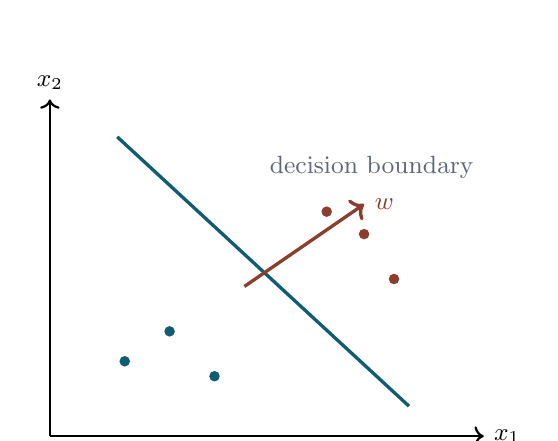
\begin{tikzpicture}[scale=0.95, every node/.style={font=\small}]
  \draw[->, thick] (0,0) -- (5.8,0) node[right] {$x_1$};
  \draw[->, thick] (0,0) -- (0,4.5) node[above] {$x_2$};
  \draw[AccentBlue, very thick] (0.9,4.0) -- (4.8,0.4);
  \node[text=Muted] at (4.3,3.6) {decision boundary};
  \draw[->, very thick, Accent] (2.6,2.0) -- (4.2,3.1) node[right] {$w$};
  \fill[AccentBlue] (1.0,1.0) circle (2pt);
  \fill[AccentBlue] (1.6,1.4) circle (2pt);
  \fill[AccentBlue] (2.2,0.8) circle (2pt);
  \fill[Accent] (4.2,2.7) circle (2pt);
  \fill[Accent] (4.6,2.1) circle (2pt);
  \fill[Accent] (3.7,3.0) circle (2pt);
\end{tikzpicture}
\end{center}

\subsection{Transfer functions}
Important transfer functions include:
\begin{itemize}[leftmargin=1.5em]
  \item linear,
  \item binary threshold,
  \item logistic / sigmoid,
  \item $\tanh$,
  \item ReLU.
\end{itemize}
Why do we care about the nonlinearity? Because it lets neurons do more than linear regression-like filtering. Nonlinear transfer functions enable classification, richer decision surfaces, and interpretable outputs such as probabilities in appropriate settings.

\subsection{Geometry to remember}
\begin{itemize}[leftmargin=1.5em]
  \item The weight vector $w$ is normal to the separating hyperplane.
  \item Changing the bias or threshold shifts the hyperplane without rotating it.
  \item The sign and magnitude of $w^\top x - \theta$ describe how strongly the input aligns with the neuron's preferred direction.
\end{itemize}

\section{Multilayer perceptrons and backpropagation}
\miheader{Why one layer is not enough}
A single linear threshold unit cannot solve non-linearly separable problems such as XOR. A multilayer perceptron (MLP) solves this by stacking multiple nonlinear units. Earlier layers transform the representation; later layers solve an easier problem in the transformed space.

\subsection{Network classes}
The lecture distinguishes two broad classes:
\begin{itemize}[leftmargin=1.5em]
  \item \textbf{Feedforward networks}: information flows from input to output.
  \item \textbf{Recurrent networks}: the graph contains cycles and internal state.
\end{itemize}
For the early foundations of the course, the emphasis is on feedforward networks.

\subsection{Universal approximation --- with a caveat}
An MLP with hidden units can approximate a broad range of functions. But expressive power is not the same as trainability. A network may be flexible enough to represent a solution while still being hard to optimize in practice.

\begin{center}
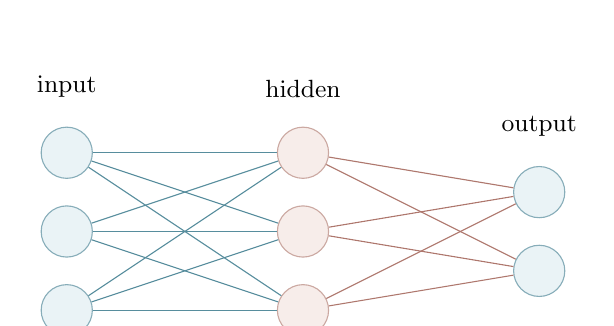
\begin{tikzpicture}[>=Latex, node distance=1.3cm, every node/.style={font=\small}]
  \node[circle, draw=AccentBlue!50, fill=SoftBlue, minimum size=0.65cm] (i1) at (0,2.2) {};
  \node[circle, draw=AccentBlue!50, fill=SoftBlue, minimum size=0.65cm] (i2) at (0,1.2) {};
  \node[circle, draw=AccentBlue!50, fill=SoftBlue, minimum size=0.65cm] (i3) at (0,0.2) {};
  \node[circle, draw=Accent!45, fill=SoftRose, minimum size=0.65cm] (h1) at (3,2.2) {};
  \node[circle, draw=Accent!45, fill=SoftRose, minimum size=0.65cm] (h2) at (3,1.2) {};
  \node[circle, draw=Accent!45, fill=SoftRose, minimum size=0.65cm] (h3) at (3,0.2) {};
  \node[circle, draw=AccentBlue!50, fill=SoftBlue, minimum size=0.65cm] (o1) at (6,1.7) {};
  \node[circle, draw=AccentBlue!50, fill=SoftBlue, minimum size=0.65cm] (o2) at (6,0.7) {};
  \foreach \src in {i1,i2,i3} {
    \foreach \dst in {h1,h2,h3} {
      \draw[AccentBlue!70] (\src) -- (\dst);
    }
  }
  \foreach \src in {h1,h2,h3} {
    \draw[Accent!70] (\src) -- (o1);
    \draw[Accent!70] (\src) -- (o2);
  }
  \node[above=0.25cm of i1] {input};
  \node[above=0.25cm of h1] {hidden};
  \node[above=0.25cm of o1] {output};
\end{tikzpicture}
\end{center}

\subsection{Backpropagation in one sentence}
Backpropagation computes how each weight influences the loss by applying the chain rule from the output layer back toward earlier layers.

\subsection{Training loop}
\begin{enumerate}[leftmargin=1.6em]
  \item Forward pass: compute activations and outputs.
  \item Compute the loss.
  \item Backward pass: propagate error signals backward.
  \item Update weights using the negative gradient.
\end{enumerate}

For any individual parameter, backpropagation answers the question:
\begin{quote}
If I change this weight slightly, how much does the final loss change?
\end{quote}
That is what makes large layered networks trainable: local derivatives can be composed into global gradients.

\subsection{Classification link}
For multi-class prediction, a standard combination is:
\begin{itemize}[leftmargin=1.5em]
  \item \textbf{softmax} at the output, to convert scores into class probabilities,
  \item \textbf{cross-entropy loss}, to penalize low probability assigned to the true class.
\end{itemize}
This pairing becomes the modern default for multi-class neural network classification.

\section{Optimization, regularization, and validation}
\miheader{Training well is not just about gradients}
Once the network architecture exists, the next question is how to train it effectively and how to prevent it from simply memorizing the training data.

\subsection{Optimization regimes}
\subsubsection{Batch gradient descent}
Uses the full dataset for each gradient step. This gives a stable estimate of the gradient but is often too expensive for large datasets.

\subsubsection{Online / stochastic gradient descent}
Uses one sample at a time. It is cheap per update but noisy, can wander around minima, and often requires learning-rate annealing.

\subsubsection{Mini-batch optimization}
This is the practical compromise and the modern standard. It is more stable than pure stochastic updates and much cheaper than full-batch training.

\subsection{Improving optimization}
The lectures emphasize several important refinements:
\begin{itemize}[leftmargin=1.5em]
  \item \textbf{Momentum / impulse terms}: smooth updates and maintain motion in consistent downhill directions.
  \item \textbf{Adaptive step sizes}: avoid using a crude fixed learning rate everywhere.
  \item \textbf{Conjugate gradient / line search ideas}: use local curvature information more intelligently.
  \item \textbf{Adam}: combine momentum-like averaging with per-parameter adaptive scaling.
\end{itemize}

\subsection{Training error vs. generalization error}
A model can fit the training data well and still fail on new data.
\begin{itemize}[leftmargin=1.5em]
  \item \textbf{Training error}: performance on observed samples.
  \item \textbf{Generalization error}: expected performance on new samples from the same data distribution.
\end{itemize}
The gap between these two quantities is the main reason regularization and validation matter.

\begin{center}
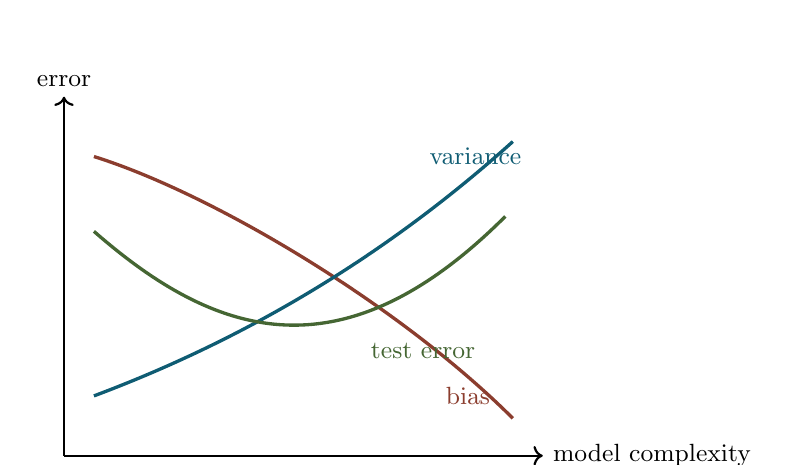
\begin{tikzpicture}[scale=0.95, every node/.style={font=\small}]
  \draw[->, thick] (0,0) -- (6.4,0) node[right] {model complexity};
  \draw[->, thick] (0,0) -- (0,4.8) node[above] {error};
  \draw[Accent, very thick] (0.4,4.0) .. controls (2.0,3.5) and (4.5,2.0) .. (6.0,0.5);
  \draw[AccentBlue, very thick] (0.4,0.8) .. controls (2.0,1.4) and (4.0,2.4) .. (6.0,4.2);
  \draw[OliveGreen!70!black, very thick] (0.4,3.0) .. controls (2.0,1.6) and (3.7,1.0) .. (5.9,3.2);
  \node[text=Accent] at (5.4,0.8) {bias};
  \node[text=AccentBlue] at (5.5,4.0) {variance};
  \node[text=OliveGreen!70!black] at (4.8,1.4) {test error};
\end{tikzpicture}
\end{center}

\subsection{Overfitting, underfitting, bias, variance}
\begin{itemize}[leftmargin=1.5em]
  \item \textbf{Underfitting}: the model is too simple; both train and test performance are poor.
  \item \textbf{Overfitting}: the model is too flexible; training performance is strong but test performance degrades.
  \item \textbf{Bias}: systematic error from models that are too rigid.
  \item \textbf{Variance}: sensitivity to the particular sampled training set.
\end{itemize}
As model complexity increases, bias tends to fall while variance tends to rise.

\subsection{Regularization tools}
\begin{conceptbox}{Weight decay}
Add a norm penalty to the objective so that large weights are discouraged. This favors simpler solutions and shrinks parameter values that are not well supported by data.
\end{conceptbox}

\begin{conceptbox}{Early stopping}
Monitor validation performance and stop training when it ceases to improve. This acts as an implicit regularizer and can prevent continued fitting of noise.
\end{conceptbox}

\begin{conceptbox}{Validation discipline}
Keep training, validation, and test roles conceptually separate: training fits parameters, validation chooses hyperparameters or stopping point, and the test set is reserved for final unbiased evaluation.
\end{conceptbox}

\begin{conceptbox}{Cross-validation}
Average validation performance across folds when data are limited to obtain a more reliable estimate of out-of-sample performance.
\end{conceptbox}

\section{Deep learning foundations}
\miheader{What changed, and why}
Deep learning is not a different philosophy from earlier machine learning topics. It extends the same pipeline --- representation, objective, optimization, and regularization --- but at greater representational depth and practical scale.

\subsection{Why deep networks originally looked difficult}
The course notes emphasize that deep multilayer perceptrons were once seen as hard to train because of:
\begin{itemize}[leftmargin=1.5em]
  \item vanishing gradients with sigmoid-like nonlinearities,
  \item long convergence times,
  \item large parameter counts,
  \item datasets that were too small,
  \item insufficient computational power.
\end{itemize}
This is why shallow methods and support vector machines dominated for a period.

\subsection{Why deep learning came back}
Several things improved together:
\begin{enumerate}[leftmargin=1.6em]
  \item larger datasets,
  \item far more compute,
  \item improved tricks of the trade,
  \item better representations learned across many layers.
\end{enumerate}
The key idea is that depth allows successive layers to build increasingly abstract features.

\subsection{Deep representations}
A deep network can form a hierarchy:
\begin{itemize}[leftmargin=1.5em]
  \item early layers capture simple local structure,
  \item middle layers combine those into motifs or parts,
  \item later layers represent task-relevant abstractions.
\end{itemize}
This helps explain why deep models can outperform shallow alternatives even when both are expressive in principle.

\subsection{Autoencoders and pre-training}
An autoencoder learns to compress and reconstruct data. The bottleneck forces a compact internal representation, which can be useful for unsupervised pre-training or initialization before fine-tuning on a downstream task.

\begin{center}
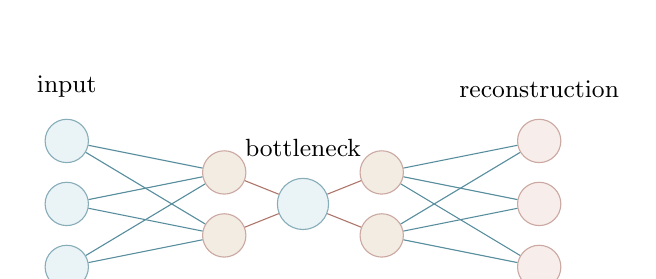
\begin{tikzpicture}[>=Latex, node distance=1cm, every node/.style={font=\small}]
  \node[circle, draw=AccentBlue!50, fill=SoftBlue, minimum size=0.55cm] (l1) at (0,2.0) {};
  \node[circle, draw=AccentBlue!50, fill=SoftBlue, minimum size=0.55cm] (l2) at (0,1.2) {};
  \node[circle, draw=AccentBlue!50, fill=SoftBlue, minimum size=0.55cm] (l3) at (0,0.4) {};
  \node[circle, draw=Accent!45, fill=SoftRose, minimum size=0.55cm] (r1) at (6,2.0) {};
  \node[circle, draw=Accent!45, fill=SoftRose, minimum size=0.55cm] (r2) at (6,1.2) {};
  \node[circle, draw=Accent!45, fill=SoftRose, minimum size=0.55cm] (r3) at (6,0.4) {};
  \node[circle, draw=Accent!45, fill=Soft, minimum size=0.55cm] (m1) at (2,1.6) {};
  \node[circle, draw=Accent!45, fill=Soft, minimum size=0.55cm] (m2) at (2,0.8) {};
  \node[circle, draw=Accent!45, fill=Soft, minimum size=0.55cm] (n1) at (4,1.6) {};
  \node[circle, draw=Accent!45, fill=Soft, minimum size=0.55cm] (n2) at (4,0.8) {};
  \node[circle, draw=AccentBlue!50, fill=SoftBlue, minimum size=0.65cm] (b) at (3,1.2) {};
  \foreach \src in {l1,l2,l3} {
    \foreach \dst in {m1,m2} {\draw[AccentBlue!70] (\src) -- (\dst);}
  }
  \foreach \src in {m1,m2} {\draw[Accent!70] (\src) -- (b);} 
  \foreach \dst in {n1,n2} {\draw[Accent!70] (b) -- (\dst);} 
  \foreach \src in {n1,n2} {
    \foreach \dst in {r1,r2,r3} {\draw[AccentBlue!70] (\src) -- (\dst);}
  }
  \node[above=0.15cm of l1] {input};
  \node[above=0.15cm of b] {bottleneck};
  \node[above=0.15cm of r1] {reconstruction};
\end{tikzpicture}
\end{center}

\subsection{Practical regularization in deep networks}
\begin{itemize}[leftmargin=1.5em]
  \item \textbf{Data augmentation}: synthesize additional plausible inputs by transforming existing examples.
  \item \textbf{Dropout}: randomly deactivate units during training to discourage co-adaptation and improve robustness.
\end{itemize}

\section{Recurrent neural networks}
\miheader{Learning from sequences instead of IID examples}
In sequence problems, samples inside one sequence are not IID. The prediction at time step $t$ depends on what came before, so the model must retain some form of memory. A fixed-window feedforward approximation conditions only on a recent context,
\[
P\bigl(y_t \mid y_{t-k},\dots,y_{t-1}\bigr),
\]
but this forces us to choose a finite horizon in advance. Recurrent neural networks replace the explicit window by a latent state that is updated over time.

\subsection{Core RNN dynamics}
A basic recurrent network processes one input at a time:
\[
s_t = f(Ux_t + Ws_{t-1} + b_s),
\qquad
y_t = g(Vs_t + b_y).
\]
Here $s_t$ is the hidden state, $U$ maps the current input into state space, $W$ carries forward the previous state, and $V$ maps state to output.

\textbf{Intuition.} The hidden state $s_t$ is a compressed memory of the past. Instead of remembering every earlier input explicitly, the network learns what should be preserved and what can be forgotten.

\subsection{Backpropagation through time}
For a sequence dataset, the cost accumulates over time,
\[
E = \frac{1}{p}\sum_{\alpha=1}^{p} \frac{1}{n_\alpha}\sum_{t=1}^{n_\alpha} e^{(\alpha,t)},
\]
so training unfolds the recurrence across time and applies backpropagation through time (BPTT).

\textbf{Intuition.} An RNN is a deep network in disguise, where the depth dimension is time. BPTT sends error signals backward through earlier hidden states that influenced the present prediction.

\subsection{Why long-term dependencies are hard}
If we linearize the recurrence, repeated application of the recurrent matrix gives
\[
s_t = W^t s_0.
\]
The same repeated multiplication appears in the gradient, which leads to the classic problems of vanishing and exploding gradients:
\begin{itemize}[leftmargin=1.5em]
  \item if the effective gain is too small, information and gradients decay exponentially;
  \item if it is too large, activity and gradients blow up.
\end{itemize}

\textbf{Intuition.} Tiny shrinkage at each step eventually becomes total forgetting; tiny amplification eventually becomes instability.

\subsection{Architectural fixes}
The lectures motivate several responses:
\begin{itemize}[leftmargin=1.5em]
  \item \textbf{Echo-state networks}: keep the recurrent reservoir fixed and only train the readout.
  \item \textbf{Leaky units}: introduce slower state averaging,
  \[
  \mu_t = \alpha \mu_{t-1} + (1-\alpha)s_{t-1}, \qquad 0<\alpha<1.
  \]
  \item \textbf{LSTM-style gating}: maintain a protected cell state and control writing, forgetting, and reading through gates,
  \[
  c_t = f_t \odot c_{t-1} + i_t \odot \tilde c_t,
  \qquad
  s_t = o_t \odot \tanh(c_t).
  \]
\end{itemize}

\textbf{Intuition.} Gating creates a memory line that can persist across many time steps without forcing every intermediate nonlinear transformation to preserve the signal.

\section{Radial basis function networks}
\miheader{Local approximation rather than global hidden features}
A radial basis function (RBF) network predicts with a linear combination of localized basis functions:
\[
y(x) = \sum_{i=1}^{M} w_i\,\phi_i(x),
\qquad
\phi_i(x)=\exp\!\left(-\frac{\lVert x-t_i\rVert^2}{2\sigma_i^2}\right).
\]
Each hidden unit is centered at a prototype $t_i$ with width $\sigma_i$.

\textbf{Intuition.} Each basis function fires only near its own center, so the network behaves like a patchwork of local experts rather than a single global feature hierarchy.

\subsection{Why RBFs are attractive}
RBF networks often learn quickly because only nearby basis functions matter strongly for a given input. But they pay for this locality with poor scaling in high dimension: to cover an $N$-dimensional space with roughly $M$ basis functions per dimension requires on the order of $M^N$ local regions.

\textbf{Intuition.} Local approximation is powerful when the data lives in low-dimensional or clustered structure, but expensive when the ambient space is large.

\subsection{Two-step learning procedure}
A practical learning pipeline is:
\begin{enumerate}[leftmargin=1.6em]
  \item choose centers $t_i$ by unsupervised learning,
  \item choose widths $\sigma_i$ heuristically,
  \item solve the output weights $w_i$ by supervised linear regression.
\end{enumerate}
Centers are often learned by online $k$-means:
\[
i = \arg\min_j \lVert x^{(\alpha)} - t_j \rVert,
\qquad
\Delta t_i = \eta_t\bigl(x^{(\alpha)} - t_i\bigr).
\]
A standard width heuristic is
\[
\sigma_i = \lambda \min_{j\neq i}\lVert t_i - t_j \rVert,
\]
with $\lambda$ chosen to ensure enough overlap between neighboring basis functions.

\subsection{Closed-form output learning}
Once the hidden features are fixed, the model is linear in $w$. With design matrix entries
\[
\Phi_{\alpha i} = \phi_i(x^{(\alpha)}),
\]
the least-squares solution satisfies the normal equations
\[
\Phi^\top \Phi \, w = \Phi^\top y_T,
\qquad
w = (\Phi^\top \Phi)^{-1}\Phi^\top y_T
\]
when the inverse exists.

\textbf{Intuition.} The hard nonlinear part is delegated to the basis functions; the final fitting step is just linear regression in the transformed feature space.

\subsection{Normalization and regularization}
A normalized RBF layer uses
\[
\psi_i(x) = \frac{\phi_i(x)}{\sum_j \phi_j(x)},
\qquad
y(x)=\sum_i w_i\psi_i(x),
\]
which turns the hidden layer into a soft interpolation over nearby prototypes. If the least-squares problem is ill-conditioned, ridge regularization gives
\[
w = (\Phi^\top \Phi + \lambda I)^{-1}\Phi^\top y_T.
\]

\textbf{Intuition.} Regularization picks smoother functions when many different local interpolants fit the same training data.

\section{Statistical learning theory}
\miheader{Why low training error is not enough}
The central question of statistical learning theory is: when does minimizing training error actually produce a predictor that generalizes? For a predictor $y(x;w)$ and loss $e(y,x;w)$, the true risk is
\[
R(w)=\int P(x,y)\,e(y,x;w)\,dx\,dy,
\]
while the empirical risk is
\[
R_{\mathrm{emp}}(w)=\frac{1}{p}\sum_{i=1}^{p} e(y_i,x_i;w).
\]
Empirical risk minimization (ERM) chooses
\[
w_p = \arg\min_w R_{\mathrm{emp}}(w).
\]

\textbf{Intuition.} ERM replaces an unknown expectation by a sample average. That replacement is only justified if the sample average is uniformly close to the true expectation across the whole model class.

\subsection{Capacity and the growth function}
Capacity is captured by the number of distinct labelings that a hypothesis class can realize on $p$ points. The growth function measures the worst-case logarithmic count of those labelings. If capacity is too high, the class can fit arbitrary labels and low training error becomes uninformative.

For linear classifiers in general position, Cover's counting argument gives the number of separable assignments:
\[
C(p,N)=2\sum_{k=0}^{N-1} \binom{p-1}{k}.
\]

\subsection{VC dimension}
The VC dimension $d_{\mathrm{VC}}$ is the largest number of points that can be shattered by the model class. A key learning-theory message is that finite VC dimension makes generalization possible. Heuristically, generalization bounds have the form
\[
R(w) \le R_{\mathrm{emp}}(w) + C\bigl(p,d_{\mathrm{VC}}\bigr),
\]
where the second term penalizes model capacity.

\textbf{Intuition.} Good learning requires both fit and restraint: a flexible enough class to represent the solution, but not so flexible that fitting the sample is trivial.

\subsection{Structural risk minimization}
Structural risk minimization (SRM) replaces ``minimize training error in one fixed class'' with ``balance training fit against complexity across nested classes.'' This is the conceptual bridge from statistical learning theory to support vector machines.

\section{Support vector machines}
\miheader{Margin maximization as capacity control}
For a linear classifier
\[
f(x)=w^\top x + b,
\qquad
y(x)=\operatorname{sign}(f(x)),
\]
the canonical normalization is chosen so that
\[
\min_i y_i(w^\top x_i + b)=1.
\]
Then the distance of the closest point to the hyperplane is proportional to $1/\lVert w\rVert$, so maximizing the margin is equivalent to minimizing $\frac12\lVert w\rVert^2$.

\textbf{Intuition.} Among all separating hyperplanes, choose the one with the widest safety buffer. A larger margin means lower effective capacity and better robustness to perturbations.

\subsection{Hard-margin primal problem}
For linearly separable data, the SVM solves
\[
\min_{w,b}\; \frac12 \lVert w \rVert^2
\]
subject to
\[
y_i(w^\top x_i+b) \ge 1,
\qquad i=1,\dots,p.
\]

\subsection{Dual formulation and support vectors}
Introducing Lagrange multipliers $\alpha_i\ge 0$ yields the dual problem
\[
\max_{\alpha}\; \sum_{i=1}^{p} \alpha_i - \frac12\sum_{i,j=1}^{p}\alpha_i\alpha_j y_i y_j\, x_i^\top x_j
\]
subject to
\[
\sum_{i=1}^{p} \alpha_i y_i = 0,
\qquad
\alpha_i \ge 0.
\]
The optimal classifier has the form
\[
w^* = \sum_{i=1}^{p} \alpha_i^* y_i x_i,
\qquad
y(x)=\operatorname{sign}\!\left(\sum_{i=1}^{p}\alpha_i^* y_i x_i^\top x + b^*\right).
\]
Only points with $\alpha_i^*>0$ remain in the final solution; these are the support vectors.

\textbf{Intuition.} Most training points disappear. The classifier is determined only by the points that sit on the margin and therefore constrain the decision boundary.

\subsection{Soft margins and kernels}
Real data are usually not perfectly separable, so slack variables $\xi_i\ge 0$ produce the soft-margin objective
\[
\min_{w,b,\xi}\; \frac12\lVert w\rVert^2 + \frac{C}{p}\sum_{i=1}^{p}\xi_i
\]
subject to
\[
y_i(w^\top x_i+b) \ge 1-\xi_i.
\]
The hyperparameter $C$ controls the trade-off between a wide margin and few violations.

In the dual, data appear only through inner products. Replacing $x_i^\top x_j$ by a kernel $k(x_i,x_j)$ gives the kernel SVM:
\[
y(x)=\operatorname{sign}\!\left(\sum_{i\in SV}\alpha_i y_i\, k(x_i,x) + b\right).
\]
Common choices include the polynomial kernel and the Gaussian kernel,
\[
k(x,x')=(x^\top x'+1)^d,
\qquad
k(x,x')=\exp\!\left(-\frac{\lVert x-x'\rVert^2}{2\sigma^2}\right).
\]

\textbf{Intuition.} The kernel trick keeps optimization linear in feature space while making the decision boundary nonlinear in the original input space.

\section{Uncertainty and inference}
\miheader{Probability as rational belief under incomplete information}
This lecture block treats probability as a calculus of plausible reasoning. A proposition $H$ is assigned a degree of belief $P(H)\in[0,1]$, and those beliefs must obey the probability axioms to remain coherent.

\subsection{Inference by marginalization and conditioning}
If $x$ is a query and $e$ is observed evidence, then
\[
P(x\mid e)=\frac{P(x,e)}{P(e)}.
\]
If there are hidden variables $y$, inference requires summing them out:
\[
P(x\mid e)=\alpha \sum_y P(x,e,y),
\qquad
\alpha^{-1}=\sum_{x,y} P(x,e,y).
\]
Bayes' rule follows from the product rule:
\[
P(Y\mid X)=\frac{P(X\mid Y)P(Y)}{P(X)}.
\]

\textbf{Intuition.} Inference means ``sum over what you do not know, then renormalize over what remains.''

\subsection{Conditional independence}
The main route to tractable probabilistic reasoning is conditional independence:
\[
X \perp Y \mid Z
\qquad \Longleftrightarrow \qquad
P(X,Y\mid Z)=P(X\mid Z)P(Y\mid Z).
\]
This is the idea that once $Z$ is known, learning $Y$ tells us nothing further about $X$.

A classic simplification is Naive Bayes,
\[
P(X_1,\dots,X_{N-1},Y)=P(Y)\prod_{i=1}^{N-1}P(X_i\mid Y),
\]
which drastically reduces complexity by assuming the observed variables become independent once the latent cause $Y$ is known.

\section{Bayesian networks}
\miheader{Encoding probabilistic structure with directed acyclic graphs}
A Bayesian network is a directed acyclic graph whose nodes are random variables and whose edges encode direct statistical dependencies. Its defining factorization is
\[
P(X_1,\dots,X_n)=\prod_{i=1}^{n} P\bigl(X_i\mid \mathrm{pa}(X_i)\bigr),
\]
where $\mathrm{pa}(X_i)$ denotes the parents of $X_i$.

\textbf{Intuition.} Instead of storing one huge joint table, we store one local conditional model per variable given only its direct causes.

\subsection{Graph structure and independence}
The graph determines which variables become independent when evidence is observed. Chains and forks are blocked by conditioning on the middle or common-cause node, while colliders behave oppositely: conditioning on a common effect can create dependence.

\subsection{Markov blankets}
For a node $A$, the Markov blanket consists of its parents, its children, and the other parents of its children. Given the Markov blanket,
\[
A \perp \text{all other nodes} \mid \mathrm{MB}(A).
\]

\textbf{Intuition.} Once you know what directly influences $A$, what $A$ influences, and who competes with $A$ in explaining those effects, the rest of the graph becomes irrelevant for predicting $A$.

\subsection{Inference in Bayesian networks}
Inference still amounts to multiplying local factors and summing out hidden variables,
\[
P(x\mid e) \propto \sum_y \prod_i P(X_i\mid \mathrm{pa}(X_i)).
\]
The graph structure makes that computation much more efficient than naive enumeration and motivates algorithms based on elimination orderings and message passing.

\section{Bayesian inference and neural networks}
\miheader{From one best model to posterior-weighted prediction}
The Bayesian viewpoint starts from a generative account of data. For supervised data $z=(x,y)$, we factor the joint distribution as
\[
p(z)=p(y\mid x)\,p(x).
\]
For regression, a simple generative model is
\[
y = y^*(x) + \eta,
\]
where $y^*(x)$ is the underlying deterministic relation and $\eta$ is noise.

\subsection{Bayesian model selection}
Competing models are compared by Bayes' rule,
\[
P(M\mid E)=\frac{P(E\mid M)P(M)}{P(E)}.
\]
The posterior favors models that both explain the evidence well and were plausible a priori.

\textbf{Intuition.} A good model is not merely one that can fit the data somewhere in parameter space; it is one under which the observed data was genuinely likely.

\subsection{Bayesian prediction}
Prediction averages over model uncertainty rather than committing to a single best model:
\[
P(y\mid x,D)=\int P(y\mid x;w)\,P(w\mid D)\,dw.
\]
For discrete model families, this becomes a posterior-weighted committee over models.

\subsection{MAP estimation and regularization}
For neural networks, if the likelihood and prior take exponential forms,
\[
P(Y\mid X;w) \propto \exp\!\bigl(-\beta E_T(w)\bigr),
\qquad
P(w) \propto \exp\!\bigl(-\alpha E_R(w)\bigr),
\]
then the posterior is proportional to
\[
P(w\mid X,Y) \propto \exp\!\bigl(-\beta E_T(w)-\alpha E_R(w)\bigr).
\]
Therefore the MAP estimate solves a regularized optimization problem,
\[
w^* = \arg\min_w \bigl(E_T(w)+\alpha' E_R(w)\bigr).
\]
For quadratic regularization, this is weight decay.

\textbf{Intuition.} Regularization is not just a computational hack; it is equivalent to imposing prior beliefs on parameters.

\section{Reinforcement learning}
\miheader{Sequential decision-making under delayed reward}
Reinforcement learning studies how an agent should act in an environment when rewards can be delayed. The standard formalism is the Markov decision process (MDP), consisting of states $x$, actions $a$, transition probabilities $P(x'\mid x,a)$, rewards $r(x,a)$, and a policy $\pi(a\mid x)$.

\subsection{Value functions and discounted return}
The value of a policy $\pi$ at state $x$ is the expected discounted return,
\[
V^\pi(x)=\mathbb{E}\!\left[\sum_{t=0}^{\infty} \gamma^t r(x_t,a_t)\;\middle|\;x_0=x,\ a_t\sim \pi(\cdot\mid x_t)\right],
\qquad \gamma\in[0,1).
\]
The Bellman equation expresses this recursively:
\[
V^\pi(x_i)=\sum_k \pi(a_k\mid x_i)r(x_i,a_k) + \gamma \sum_{j,k}\pi(a_k\mid x_i)P(x_j\mid x_i,a_k)V^\pi(x_j).
\]

\textbf{Intuition.} A state is valuable if it gives reward now or tends to lead to valuable states later.

\subsection{Temporal-difference learning}
Monte Carlo evaluation waits for full returns. Temporal-difference learning bootstraps from the next estimate:
\[
\tilde V_{t+1}(x_t)=\tilde V_t(x_t)+\eta\Bigl[r_t + \gamma \tilde V_t(x_{t+1}) - \tilde V_t(x_t)\Bigr].
\]
The bracketed term is the TD error.

\textbf{Intuition.} TD learning updates immediately by treating the next prediction as a temporary target, rather than waiting until the end of the episode.

\subsection{Q-values and control}
For action selection we need values of state-action pairs:
\[
Q^\pi(x_i,a_k)=r(x_i,a_k)+\gamma\sum_j P(x_j\mid x_i,a_k)V^\pi(x_j),
\qquad
V^\pi(x)=\sum_a \pi(a\mid x)Q^\pi(x,a).
\]
A greedy policy chooses the action with largest Q-value.

\subsection{SARSA and Q-learning}
SARSA is on-policy:
\[
Q_{t+1}(x_t,a_t)=Q_t(x_t,a_t)+\eta\Bigl[r_t+\gamma Q_t(x_{t+1},a_{t+1})-Q_t(x_t,a_t)\Bigr].
\]
Q-learning is off-policy:
\[
Q_{t+1}(x_t,a_t)=Q_t(x_t,a_t)+\eta\Bigl[r_t+\gamma\max_{a'}Q_t(x_{t+1},a')-Q_t(x_t,a_t)\Bigr].
\]

\textbf{Intuition.} SARSA learns the value of the policy the agent is actually following; Q-learning learns the value of acting optimally from the next step onward even while the behavior policy remains exploratory.

\subsection{Exploration versus exploitation}
The agent must balance trying uncertain actions against exploiting currently good ones. Standard choices include $\varepsilon$-greedy exploration and softmax action selection,
\[
\pi(a\mid x) = \frac{\exp\bigl(\beta Q(x,a)\bigr)}{\sum_{a'} \exp\bigl(\beta Q(x,a')\bigr)}.
\]

\textbf{Intuition.} Without exploration, the agent can get stuck with a locally good but globally poor strategy; without exploitation, it never benefits from what it has learned.

\section{Cross-topic synthesis}
\miheader{One storyline, not isolated lecture blocks}
The complete course fits together as one argument:
\begin{enumerate}[leftmargin=1.6em]
  \item \textbf{Learning foundations} define model classes, objectives, and training procedures.
  \item \textbf{Neural network models} build expressive function approximators from neurons, hidden layers, recurrent state, and localized basis functions.
  \item \textbf{Learning theory} explains when low training error can be trusted and why capacity control matters.
  \item \textbf{Large-margin methods} turn those ideas into concrete optimization principles via support vector machines.
  \item \textbf{Probabilistic reasoning} handles uncertainty through structured distributions, Bayesian updating, and model averaging.
  \item \textbf{Reinforcement learning} extends prediction to sequential control under delayed reward.
\end{enumerate}

\begin{summarybox}
\textbf{If you only remember twelve things:}
\begin{enumerate}[leftmargin=1.6em]
  \item Machine learning can be framed as model selection.
  \item A neuron is a weighted sum followed by a nonlinearity.
  \item Hidden state is the key to sequence modeling.
  \item RBF networks approximate locally, not globally.
  \item Training error and generalization error are not the same thing.
  \item Capacity control is the central theme of statistical learning theory.
  \item Margins connect geometry to generalization.
  \item SVMs solve structural risk minimization in optimization form.
  \item Bayesian reasoning updates prior beliefs with evidence.
  \item Graph structure can make high-dimensional inference tractable.
  \item Regularization can be interpreted as a prior over parameters.
  \item Reinforcement learning is value-based reasoning over future reward, not just immediate reward.
\end{enumerate}
\end{summarybox}

\section*{Primary sources used}
\addcontentsline{toc}{section}{Primary sources used}
\begin{itemize}[leftmargin=1.5em]
  \item \texttt{Lecture Slides/11-Introduction.pdf}
  \item \texttt{Lecture Slides/12-Connectionist Neurons.pdf}
  \item \texttt{Lecture Slides/13-Multilayer Perceptrons.pdf}
  \item \texttt{Lecture Slides/14-Additional Topics.pdf}
  \item \texttt{Lecture Slides/15-Deep Learning.pdf}
  \item \texttt{Lecture Slides/16-Recurrent Neural Networks.pdf}
  \item \texttt{Lecture Slides/17-Radial Basis Function Networks.pdf}
  \item \texttt{Lecture Slides/21-Elements of Statistical Learning Theory.pdf}
  \item \texttt{Lecture Slides/22-Support Vector Machines.pdf}
  \item \texttt{Lecture Slides/31-Uncertainty and Inference.pdf}
  \item \texttt{Lecture Slides/32-Bayesian Networks.pdf}
  \item \texttt{Lecture Slides/33-Bayesian Inference and Neural Networks.pdf}
  \item \texttt{Lecture Slides/41-Reinforcement Learning - Valuation.pdf}
  \item \texttt{Lecture Slides/42-Reinforcement Learning - Policy Learning.pdf}
  \item Existing Obsidian lecture and tutorial notes for the corresponding topics
\end{itemize}

\end{document}
